%author Luis Alberto Martinez Monroy
%Materia Estructuras Discretas 2017-1
%Numero de cuenta: 314212391
%Practica de Laboratorio #1
%Profesora: Laura Freidberg Gojman
%Ayudante de laboratorio: Albert Manuel Orozco Camacho
%Facultad de ciencias

\documentclass{report}%tipo de documento.
\textheight=25cm % delimitado el alto del area de impresion
\textwidth=15cm % delimitado lo ancho del area de imprecion
\topmargin=-3cm % delimita el margen superior
\setlength{\columnsep}{7mm}


\usepackage[spanish]{babel}% paquete para lengua en español
\usepackage[utf8]{inputenc}%paquete para poner acentos, etc.
\usepackage{graphicx} %Paquete para incluir graficos e imagenes
\usepackage[T1]{fontenc}%tipo de letra
% paquete para cabezera y pie de pagina.
\usepackage{lastpage}%Hace referencia al numero de paginas
\usepackage{ifthen}
\usepackage{amsmath,amsfonts,amsthm} %paquetes matematicos
\usepackage{sfmath} % paquetes matematicos
\usepackage{anyfontsize} %paquete para tamaño de texto
\usepackage{hyperref} %Paquete para hipervinculo
\usepackage{multicol} % Paquete para multicolumna
\usepackage{listings} %Paquete para mostrar codigo
\usepackage[rightcaption]{sidecap}
\DeclareGraphicsExtensions{,.pdf,.png,.jpg,.gif}
\usepackage{epstopdf}
\graphicspath{ {images/} }

\begin{document} % inicia el contenido de mi documento

\thispagestyle{plain}%tipo de la hoja
               \titlehead% Esto es para poner algunos datos como la escuela, prof, etc.
                   {
                     Materia: Estructuras Discretas 2017-1\\
                     Profesora: Laura Freudberg Gojman\\
                     Universidad Nacional Autonoma De México\hfill
                     Facultad de ciencias\\
                     Alumno: Luis Alberto Martinez Monroy
                   }


\begin{center}% No funciono \title y \subtitle asi que esta es la representacion de mi titulo y mi subtitulo buscando alternativas.

{\Huge Practica #3 Estructuras Discretas\\}\\% Este es el Titulo
{\Large Practica para desarrollar empleo de columnas, etc.}\\\\% Este es el subtitulo
\hrule\\%Esta es la linea que aparece despues del subtitulo

\end{center}
\vspace{.3cm} %espaciado vertical 
\begin{center}%Para centrar mi nombre y la fecha despues del espaciado
Alumno: Luis Alberto Martinez Monroy\\\\% Nombre de alumno
N Cuenta: 314212391\\\\%Numero de cuenta

\begin{tabular}{cc}%fecha de entrega, pero lo puse como en tabla para que se viera muy bonito y sin lineas
                       \textsc{Fecha de entrega:}& \textsc{28 de agosto 2016}\\
                   \end{tabular}

\end{center}% termina el centrado de nombre y fecha
\Seccion{{\Large Actividades}}\\%formato titulo de secciones
\subseccion{\Large Actividades.-1-6: Las actividades del 1-6 ya las he entregado anteriormente con la practica 2.}\\
\subseccion{{\large7.-resumen del articulo: \href{https://medium.com/@jugoncalves/ \\functional-programming-should-be-your-1-priority-for\\-2015-47dd4641d6b9#.rkhnqd90r}{PROGRAMACION FUNCIONAL}}}\\

\begin{multicols}{2}
{\normalsize
El articulo habla acerca de las caracteristicas que se tienen al utilizar la programacion funcional, pero antes de llegar a esto, nos dice que que si \"{googleamos: PROGRAMACION FUNCIONAL}, no encontraremos nada nuevo en comparacion de lo que se definió a principios de los 50.\\
Se puede entender la PROGRAMACION FUNCIONAL como programacion pero utilizando funciones, de tal manera que se puden utilizar esas funciones para hacer composicion de funciones y llevar el programa a una mayor complejidad.
Las cinco caracteristicas que se tienen al utilizar la programacion funcional son:\\
\begin{itemize}
  \item Funciones de Primera-Clase
  \item Funciones de Alto-Orden
  \item Funciones Puras
  \item Cierres
  \item Estados Inmutables
\end{itemize}
(**** Todos los ejemplos estan en JavaScript****)
 Funciones de Primera-Clase: Significa que puedes almacenar funciones en una variable como en el siguite ejemplo:\\
\begin{lstlisting}[JavaScript]
var add = function(a, b){
  return a + b
} 
\end{lstlisting}
 Funciones de Alto-Orden: Significa que puede regresar funciones o recibir otras funciones como parametro, como se muestra en el siguiente ejemplo:\\
 \begin{lstlisting}[JavaScript]
 document.querySelector('#button')
  .addEventListener('click', function(){
    alert('yay, i got clicked')
  }) 
 \end{lstlisting}
 Funciones Puras: Son funciones que solo reciben y envian informacion, no modifican ningun valor, no causa ningun cambio en alguna otra aparte del programa.\\
 Cierres significan que pudes ahorrate algunos valores que dentro de una funcion que solo 
Menciona tambien que pues no es facil al principio leer la sintaxis de la programacion funcional, puesto que es muy pobre en comparacion con la programacion orientada a objetos.\\

El Estado Inmutable es cuando no puedes cambiar el estado de una variable, y por lo tanto la unica manera de modificarlo, es creando un nuevo estado.\\

Por ultimo solo añadire que es muy parecido a la programacion orientada a objetos, sin embargo, se ve mucho potencial en la composicion de las funciones, y al momento de hacer esto puedes crear una complejidad en el programa, mas allá de lo que a simple vista puede parecer la programacion funcional.
}
\end{multicols}
\newpage
\thispagestyle{plain}
\subseccion{\Large 8.- Reseña de \href{http://www.aprendehaskell.es/content/Introduccion.html}{Haskell}}\\

{\normalsize
El documento, es una guia para aprender a usar HASKELL, pero no solo eso, en realidad esto solo es la introduccion, nos dice que Haskell es un lenguaje funcional, y dice que este es un lenguaje de programacion, ya que no calcula datos hasta que lo forzas a hacerlo, de tal manera tienes que estarlo presionando para que calcule resultado.\\
Por otro lado tambien podemos decir que este lenguaje puede llegar a ser muy complejo debido a que puedes unir funcion simples, para crear funciones mas complejas (composicion de funciones), y aparte de todo eso, tiene un compilador muy riguroso, al cual le permite detectar si los tipos de variable que estas utilizando son cadenas, numeros enteros, etc; Por tal motivo este es un lenguaje de programacion que a mi perspectiva es muy completo y tambien ilustro dentro de este pequeño texto lo del estado inmutable, al decir que cuando tu le asignas un valor X a la variable Y, ésta siempre sera X, porque ya habias dicho que es X.
}\\

\begin{minipage}[b]{0.4\textwidth}

                        \begin{center}
                        
\includegraphics[width=6cm]{//home/huicho/Documentos/Estructuras/Laboratorio/Practica3/img/flojera.jpg}
                       \end{center}
                       \caption{{\small Figura 1: Sólo es para representar que Haskell es flojo}}
                        
                      
\end{minipage}\hfill \begin{minipage}[b]{0.4\textwidth}
                        \begin{center}
                        
                        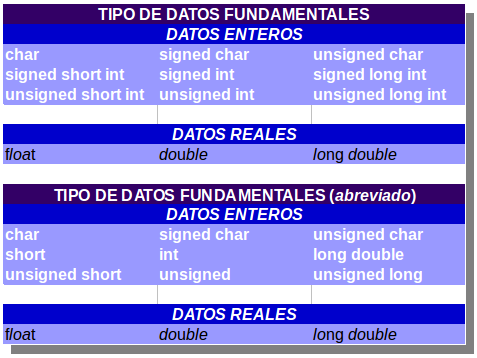
\includegraphics[width=6cm]{/home/huicho/Documentos/Estructuras/Laboratorio/Practica3/img/datos.png}

                        \end{center}
                        \caption{{\small Figura 2: Haskell puede detectar automaticamente los tipos de datos}}


                        \end{minipage}

\subseccion{{\Large 8.1- punto extra, investigacion del personaje}}\\
{\small El personaje es Richard Stallman, los aportes que ha la computacion, es la creacion del la fundacion del sofware libre y apoyo el proyecto del GNU, aparte de todo esto creo el editor de texto EMACS}

\subseccion{{\Large 9.- Explicacin de codigo de la primera practica de ICC}}\\
{\small
El Programa es el de RFC, que consiste en crear el RFC de un usuario obteniendo datos como:\\
\begin{itemize}
  \item Nombre completo del individuo.
  \item Fecha de nacimiento del individuo
\end{itemize}

Empezamos con la linea de codigo 7.- donde importaremos el objeto Scanner a nuestro programa para poder obtener datos del usuario ingresados en la consola.\\
\lstinputlisting[language = Java,  basicstyle=\small ,firstline=7, lastline=7]{/home/huicho/Documentos/Estructuras/Laboratorio/Practica3/java/RFC.java}

En la linea 9, declaramos la clase del programa que en este caso es RFC:\\
\lstinputlisting[language = Java,  basicstyle=\small ,firstline=9, lastline=9]{/home/huicho/Documentos/Estructuras/Laboratorio/Practica3/java/RFC.java}

En la linea 14, declaramos el metodo principal del programa, o el metodo MAIN:\\
\lstinputlisting[language = Java,  basicstyle=\small ,firstline=14, lastline=14]{/home/huicho/Documentos/Estructuras/Laboratorio/Practica3/java/RFC.java}


Ahora en la linea de la 15 a la 18 realizamos dos cosas, en la linea 15, creamos un objeto de la clase escaner y despues, creamos 2 variables String, con los cuales los usaremos despues para asignarles el valor de usuario.\\
\lstinputlisting[language = Java,  basicstyle=\small ,firstline=15, lastline=18]{/home/huicho/Documentos/Estructuras/Laboratorio/Practica3/java/RFC.java}

Nos situamos en la linea 20-23, donde utilizamos el comando System.out para imprimir en la pantalla del usuario, para pedirle que ingrese sus datos, ya sea fecha de nacimiento o nombre, y aqui utilizamos las variables Strings que ya habiamos creado y les asignamos como valor lo que recoja el escaner de igual manera en String.\\
\lstinputlisting[language = Java,  basicstyle=\small ,firstline=20, lastline=23]{/home/huicho/Documentos/Estructuras/Laboratorio/Practica3/java/RFC.java}

En la linea 25 a 29,realizamos 4, operaciones, medimos la longitud de nuestra cadena orginal, despues le decimos al programa que nos devuelva la cadena pero despues del primer espacio de izquierda a derecha, por penultimo paso pero no menos importante, le restamos a la longitud, la cadena despues del espacio.

Y a eso le sacamos las 2 primerar letras que corresponderian a las primeras 2 iniciales del apellido paterno.\\
\lstinputlisting[language = Java,  basicstyle=\small ,firstline=25, lastline=29]{/home/huicho/Documentos/Estructuras/Laboratorio/Practica3/java/RFC.java}

de la misma mandera lo haremos para restarle las iniciales del apellido materno, pero esta vez, trabajaremos con la cadena que se imprime despues del primer espacio. y esto es en la linea 34 a 38\\
\lstinputlisting[language = Java,  basicstyle=\small ,firstline=34, lastline=38]{/home/huicho/Documentos/Estructuras/Laboratorio/Practica3/java/RFC.java}

ya casi para terminar realizamos lo mismo que para el apellido materno pero con la cadena despues del 2 espacio, para obtener las iniciales del primer nombre.\\

\lstinputlisting[language = Java,  basicstyle=\small ,firstline=41, lastline=47]{/home/huicho/Documentos/Estructuras/Laboratorio/Practica3/java/RFC.java}

y ya estamos apunto de acabar,declaramos las variables que usaremos de la fecha y las unimos a la cadena rfcf, donde la cadena rfc2 es la fecha de nacimiento, rfc1 es los valores de las iniciales de apellido paterno, materno y nombre, y por ultimo añadiremos los ultimos tres digitos del RFC.\\
\lstinputlisting[language = Java,  basicstyle=\small ,firstline=50, lastline=62]{/home/huicho/Documentos/Estructuras/Laboratorio/Practica3/java/RFC.java}

Y por ultimo terminamos imprimiento el RFC en mayusculas, con el comando de System.out para mostrarlo al usuario en pantalla.\\

\lstinputlisting[language = Java,  basicstyle=\small ,firstline=63, lastline=63]{/home/huicho/Documentos/Estructuras/Laboratorio/Practica3/java/RFC.java}


}
\newpage
\thispagestyle{plain}
\subseccion{{\Large 10.- Tabla de verdad de la siguiente expresion}}\\
{\small
$$((p\wedge q)\vee \neg r \rightarrow s \wedge q) \leftrightarrow \neg r \vee p $$
}

\begin{tabular}{|c|c|c|c|c|c|c|c|c|c|c|c|} \hline
$p$ & $q$ & $r$ & $s$ & $p\wedge q$ & $\vee$ & $\neg r$ & $\rightarrow$ & $s\wedge q$ & $\leftrightarrow$ & $\neg s \vee p$ \\ \hline
V & V & V & V & V & V & F & V & V & V & V \\ \hline
V & V & V & F & V & V & F & F & F & F & V \\ \hline 
V & V & F & V & V & V & V & V & V & V & V \\ \hline
V & V & F & F & V & V & V & F & F & F & V \\ \hline
V & F & V & V & F & F & F & V & F & V & V \\ \hline
V & F & V & F & F & F & F & V & F & V & V \\ \hline
V & F & F & V & F & V & V & F & F & F & V \\ \hline
V & F & F & F & F & V & V & F & F & F & V \\ \hline
F & V & V & V & F & F & F & V & V & F & F \\ \hline
F & V & V & F & F & F & F & V & F & F & F \\ \hline
F & V & F & V & F & V & V & V & V & V & V \\ \hline
F & V & F & F & F & V & V & F & F & F & V \\ \hline
F & F & V & V & F & F & F & V & F & F & F \\ \hline
F & F & V & F & F & F & F & V & F & F & F \\ \hline
F & F & F & V & F & V & V & F & F & F & V \\ \hline
F & F & F & F & F & V & V & F & F & F & V \\ \hline

\end{tabular}

\begin{thebibliography}{10}% esta es la parte de la bibliografia
\bibitem{Programacion funcional}{\texttt{https://medium.com/@jugoncalves/\\functional-programming-should-be-your-1-priority-for-2015-47dd4641d6b9#.rrkpuf9kk}\\ \texsc{Consultado por ultima vez el 21 de Septiembre del 2016}}\\
% fue un pequeño problema poner el url de las paginas, pero al final pude con el comando \texttt.

\bibitem{Haskell}{\texttt{http://www.neoteo.com/la-sucesion-de-fibonacci-en-la-naturaleza}\\ \texsc{Consultado por ultima vez el 21 de Septiembre del 2016}}\\

\bibitem{imagen del panda}{\texttt{http://memeschistosos.net/wp-content/uploads/2016/06/\\memes-de-flojera-panda-con-flojera.jpg}\\ \texsc{Consultado por ultima vez el 23 de Septiembre del 2016}}\\

\bibitem{imagen de tipos de datos}{\texttt{https://baulderasec.files.wordpress.com/2014/08/\\tipodatos_1.png?w=640}\\ \texsc{Consultado por ultima vez el 23 de Septiembre del 2016}}\\
\end{thebibliography}% termina el formato de bibliografia
\end{document}%termina todo el contenido de mi documento.
